\begin{pycode}

\end{pycode}


\section{Séance 3 - Caractérisation du démodulateur seul}

\subsection{Objectifs}

    L'objectif de la séance est d'observer le comportement du démodulateur par le biais du
    multiplicateur et du filtre passe-bas ;

    \insererfigure{Images/Seance3/Schs3.jpg}{5cm}{Schéma avec multiplicateur et filtre}{Sch3s}
  

\subsection{Théorie}

\subsubsection{Le multiplicateur}

\insererfigure{Images/Seance3/Mult.jpg}{3cm}{Schéma du multiplicateur}{Mult}

Comme montré sur le schéma ci-dessus (cf. fig. \ref{fig: Mult}), le rôle du multiplicateur
est de multiplier le signal $U_{mod}$ par la valeur du sélecteur. La sélection se fait par l'envoi
d'un signal carré $U_p$ vers le sélecteur qui prend la valeur :

\begin{itemize}
    \item A : +1 quand l'amplitude max du signal est maximale;
    \item B : -1 quand l'amplitude du signal carré est nulle. 
\end{itemize}

\subsubsection{Le filtre}

Le filtre passe-bas a plusieurs utilités :

\begin{itemize}
    \item Il supprime la composante 2$f_0$ provenant de la multiplication;\\
   $ A \sin(\omega t) \cdot \sin(\omega t) = \frac{A}{2} \left( \cos(\varphi) - \cos(2\omega t + \varphi) \right)$
    \item Il supprimes des harmoniques du signal carré;
    \item Il diminue le bruit en ne laissant que la bande passante utile.
    
\end{itemize}



\subsection{Méthode}\label{montage}

\subsubsection{Multiplicateur}
\begin{itemize}
    \item Montage :
    \begin{itemize}
        \item Le jumper J6 doit être monté;
        \item Le jumper J3 doit être positionné sur les pins 2 et 3 du PCB;
        \item Brancher la sortie $U_{mult}$ à l'oscilloscope;
        \item Alimenter le PCB à -12 et 12 V;
        \item Alimenter $U_{mod}'$ avec un sinus 1 Vp;
        \item Alimenter $U_{p}$ avec un signal carré 0-5 V.
    \end{itemize}

    \insererfigure{Images/Seance3/Mt2.jpg}{5cm}{Montage réalisé}{Mt}

    \item Mesures :
    \begin{enumerate}
        \item Régler le signal $U_{mod}'$ à 100 kHz;
        \item Faire varier le déphasage de $U_{p}$ de 0 à 180° par pas de 20°;
        \item Réeffectuer l'étape 2 pour une fréquence  $U_{mod}'$ de 300 kHz.
    \end{enumerate}

\end{itemize}

\subsubsection{Filtrage}

\begin{itemize}
    \item Montage :
    \begin{itemize}
        \item Réaliser le montage du filtre ci-dessous;
        \item $R_{14}$ = 0 et $C_6$ = nc;
        \item $R_{10}$ = $R_{13}$ = $\approx$ 10 k$\Omega$.
    \end{itemize}

    \insererfigure{Images/Seance3/Filtre.jpg}{4cm}{Filtre RC}{Filtre}
Il serait possible d'obtenir un filtre d'ordre 2. Pour cela, il est nécessaire de redimensionner les 
deux résistances et les deux condensateurs, pour un filtre de Butterworth par exemple.\\

    \item Mesures :
    \begin{enumerate}
        \item Relever la tension $U_{out}$ du démodulateur sur le multimètre, pour les mêmes déphasages
        que pour la manipulation précédente.
        
    \end{enumerate}
\end{itemize}

\subsection{Multiplicateur}

Cette section présente les captures des signaux observés à l'oscilloscope. Il a été décidé de
ne montrer que les déphasages de 0° 60° 120° et 180° afin de ne pas surcharger le rapport.
 Sur les représentations, \textcolor{blue}{$U_{mult}$} est sur le channel 2, 
 \textcolor{magenta}{$U_{mod}'$} le 3 et \textcolor{green}{$U_{p}$} sur le 4. 

\subsubsection{Fréquence de 100 kHz}



\begin{figure}[H]
    \begin{minipage}[c]{.50\linewidth}
        \centering
        \rotatebox{0}{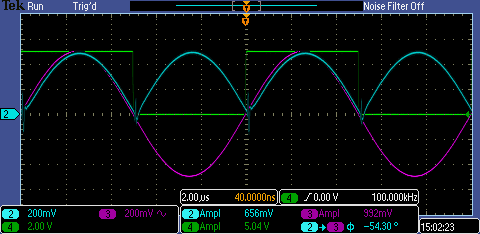
\includegraphics[scale=0.4]{Images/Seance3/partie1/TEK00000.PNG}}
        \caption{$U_{p}$, $U_{mod}'$ et $U_{mult}$ avec un\\ déphasage de 0° à 100 kHz }
    \label{fig:oc11}
    \end{minipage}
    \hfill%
    \begin{minipage}[c]{.50\linewidth}
        \centering
        \rotatebox{0}{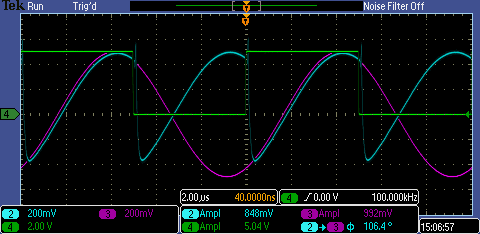
\includegraphics[scale=0.4]{Images/Seance3/partie1/TEK00003.PNG}}
       \caption{$U_{p}$, $U_{mod}'$ et $U_{mult}$ avec un \\ déphasage de 60° à 100 kHz}
 \label{fig:oc12}
    \end{minipage}
\end{figure}

\begin{figure}[H]
    \begin{minipage}[c]{.50\linewidth}
        \centering
        \rotatebox{0}{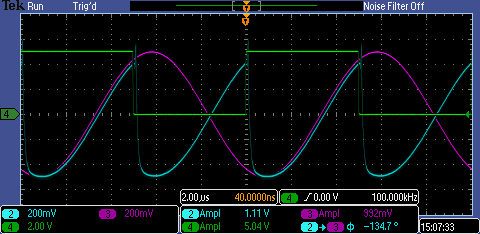
\includegraphics[scale=0.4]{Images/Seance3/partie1/TEK00006.PNG}}
        \caption{$U_{p}$, $U_{mod}'$ et $U_{mult}$ avec un\\ déphasage de 120° à 100 kHz }
    \label{fig:oc13}
    \end{minipage}
    \hfill%
    \begin{minipage}[c]{.50\linewidth}
        \centering
        \rotatebox{0}{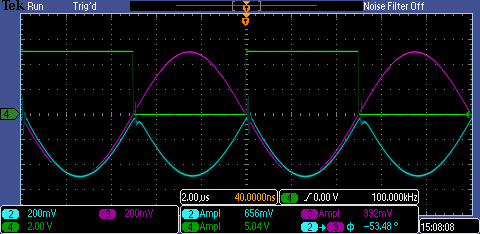
\includegraphics[scale=0.4]{Images/Seance3/partie1/TEK00009.PNG}}
       \caption{$U_{p}$, $U_{mod}'$ et $U_{mult}$ avec un \\ déphasage de 180° à 100 kHz}
 \label{fig:oc14}
    \end{minipage}
\end{figure}


\subsubsection{Fréquence de 300 kHz}


\begin{figure}[H]
    \begin{minipage}[c]{.50\linewidth}
        \centering
        \rotatebox{0}{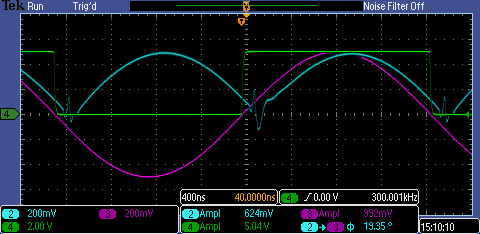
\includegraphics[scale=0.4]{Images/Seance3/partie1/TEK00010.PNG}}
        \caption{$U_{p}$, $U_{mod}'$ et $U_{mult}$ avec un\\ déphasage de 0° à 300 kHz }
    \label{fig:oc21}
    \end{minipage}
    \hfill%
    \begin{minipage}[c]{.50\linewidth}
        \centering
        \rotatebox{0}{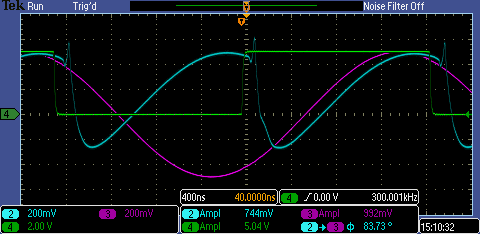
\includegraphics[scale=0.4]{Images/Seance3/partie1/TEK00013.PNG}}
       \caption{$U_{p}$, $U_{mod}'$ et $U_{mult}$ avec un \\ déphasage de 60° à 300 kHz}
 \label{fig:oc22}
    \end{minipage}
\end{figure}

\begin{figure}[H]
    \begin{minipage}[c]{.50\linewidth}
        \centering
        \rotatebox{0}{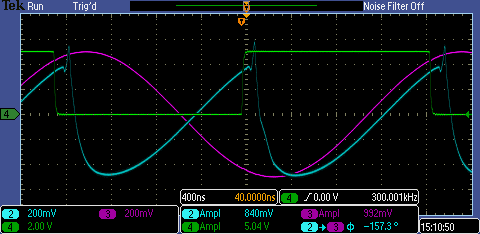
\includegraphics[scale=0.4]{Images/Seance3/partie1/TEK00016.PNG}}
        \caption{$U_{p}$, $U_{mod}'$ et $U_{mult}$ avec un\\ déphasage de 120° à 300 kHz }
    \label{fig:oc23}
    \end{minipage}
    \hfill%
    \begin{minipage}[c]{.50\linewidth}
        \centering
        \rotatebox{0}{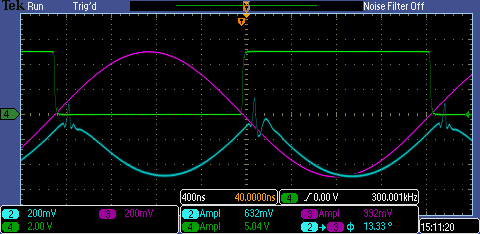
\includegraphics[scale=0.4]{Images/Seance3/partie1/TEK00019.PNG}}
       \caption{$U_{p}$, $U_{mod}'$ et $U_{mult}$ avec un \\ déphasage de 180° à 300 kHz}
 \label{fig:oc24}
    \end{minipage}
\end{figure}

\subsubsection{Analyse}

Les représentations permettent d’observer l’effet du multiplicateur  
décrit au point 4.2.1, puisque le signal \( U_{mult} \) s’inverse lors du passage à zéro du signal carré.  
Cette inversion se produit indépendamment de la valeur du déphasage. \\

Des différences apparaissent toutefois entre les séries de mesures à 100~kHz et à 300~kHz. \\  
À 300~kHz, l’électronique peine à suivre : le signal \( U_{mult} \) est déphasé par rapport au signal \( U_{mod}' \),  
et de fortes aberrations sont visibles lors des flancs du signal \( U_{p} \) en raison du slow rate et 
du filtre passe bas. \\  
Une fréquence de 300~kHz est donc trop élevée pour ce système, ce qui justifie  
l’utilisation d’une fréquence de 150~kHz pour les manipulations précédentes.


\subsection{Filtrage}

\subsubsection{Représentation des signaux}

Ci-dessous sont représentés les signaux aux différents déphasages relevés à l'oscilloscope. 

\begin{figure}[H]
    \begin{minipage}[c]{.50\linewidth}
        \centering
        \rotatebox{0}{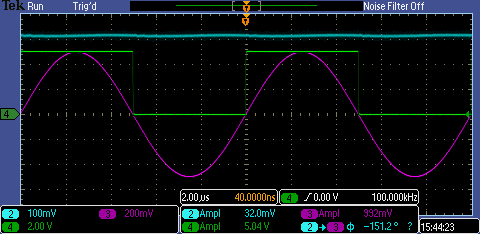
\includegraphics[scale=0.4]{Images/Seance3/partie2/TEK00000.PNG}}
        \caption{Filtre avec RC avec déphasage de 0° }
    \label{fig:f1}
    \end{minipage}
    \hfill%
    \begin{minipage}[c]{.50\linewidth}
        \centering
        \rotatebox{0}{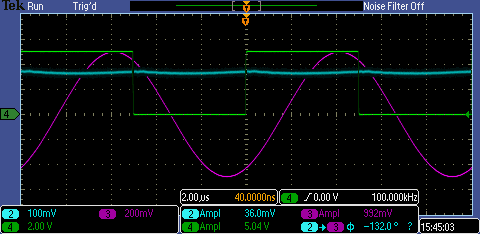
\includegraphics[scale=0.4]{Images/Seance3/partie2/TEK00003.PNG}}
       \caption{Filtre avec RC avec déphasage de 60°}
 \label{fig:f2}
    \end{minipage}
\end{figure}

\begin{figure}[H]
    \begin{minipage}[c]{.50\linewidth}
        \centering
        \rotatebox{0}{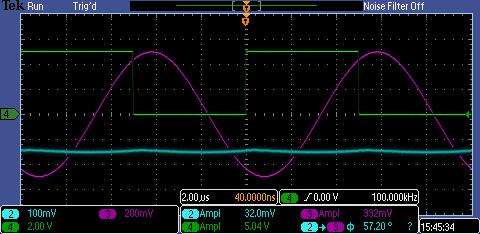
\includegraphics[scale=0.4]{Images/Seance3/partie2/TEK00006.PNG}}
        \caption{Filtre avec RC avec déphasage de 120°}
    \label{fig:f3}
    \end{minipage}
    \hfill%
    \begin{minipage}[c]{.50\linewidth}
        \centering
        \rotatebox{0}{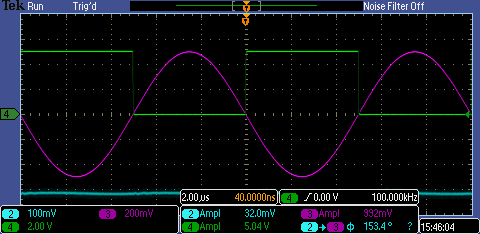
\includegraphics[scale=0.4]{Images/Seance3/partie2/TEK00009.PNG}}
       \caption{Filtre avec RC avec déphasage de 180°}
 \label{fig:f4}
    \end{minipage}
\end{figure}

Les captures ci-dessus montre la tension continue de sortie attendue et illustrent une diminution de 
celle-ci à mesure que le déphasage
 augmente, avec une amplitude maximale positive à 0° et maximale négative à 180°.

\subsubsection{Signal de sortie}


\insererfigure{Images/Seance3/Uout.png}{7cm}{Tension de sortie théorique et mesurée}{Mt}

La tension de sortie mesurée est représentée avec la tension de sortie théorique. Il est possible
de voir que les deux courbes ont la même allure, celle d'un cosinus. Cependant, l'amplitude de 
tension mesurée est inférieure à celle calculée. Cette différence pourrait s'expliquer par une 
imperfection de démodulateur.

\subsection{Conclusion}

Cette dernière séance a fourni des résultats qui correspondent aux comportements énoncés dans la 
partie théorique.\\

Résumer des résultats :

\begin{itemize}
    \item Le fonctionnement du multiplicateur a pu être observé;
    \item 300 kHz est une fréquence trop haute pour ce système;
    \item La tension de sortie du démodulateur est continue et suit l'allure d'un cosinus pour une 
    variation de déphasage.
\end{itemize}